\chapter{Architecture}
\label{chapter:dynamic resource}
This section illustrates and describes the high level architecture of the software implemented along with a few protocol sequence diagrams. It will help to understand at a high level about the components which form a part of this system to support invasive resource management and how will they interact with each other in order to integrate such an invasive resource management into existing batch systems. The following page shows the software architecture for how invasive resource management can be supported with SLURM and how exactly the new components fit into the existing software hierarchy.
\begin{itemize}
\item The top layer is that of the core resource management component which has access to job queues. In this architecture, it will now have access to not only the queue for the legacy(static) jobs but also invasive job queue(jobs submittted to invasic partition).
\item In a traditional setup the top layer will perform the task of job scheduling as well. This means that it will select a job(s) from the queue of jobs based on the current state of resources and many other factors to dispatch it to the traditional process manager below in the hierarchy. The process manager then takes the responsibility of launching these jobs on the allocated resources in the partition and managing them for their full lifetime. In case of parallel jobs, it will manage the job in a parallel environment along with facilitating the communication amongst the parallel tasks/processes with the help of a PMI(Process Manager Interface). The process manager may also spawn slave daemons on each of the nodes which are a part of the resource allocation for a single job to manage them more effectively.
\begin{figure}[!htbp]
\centering
\includegraphics[width=1.0\textwidth, height=185mm]{./figures/"iRM Architecture".pdf}
%\includegraphics[width=1.0\textwidth, height=185mm]{./figures/"software architecture".eps}
\caption{Invasive Resource Management Architecture}
\label{fig:7}
\end{figure}
\item As discussed in the previous chapter, an independent invasive resource management component by the name "iRTSched" will be implemented which needs to communicate with the batch scheduler and influence the scheduling decisions taken by it. The iRTSched sits between the top layer and the process manager.
\item A new job scheduler specifically for invasive jobs needs to be integrated into the existing batch system. In case of SLURM which has a modular design with several optional plugins, a new plugin by name "iBSched" will be implemented for SLURM to handle job scheduling specifically for invasic jobs.
\item Communication between iRTSched and iBSched will involve the negotiation protocol as explained in the previous chapter but will also include periodic / event-driven feedbacks being sent by iRTSched to iBSched. These will contain some useful information about the current state of the running jobs, their energy consumption, other job characteristics etc. This communication will also additionally support a means to service urgent jobs immediately.
\end{itemize}
%\begin{figure}[!htbp]
%\centering
%\includegraphics[width=1.0\textwidth, height=185mm]{./figures/"iRM Architecture".pdf}
%\includegraphics[width=1.0\textwidth, height=185mm]{./figures/"software architecture".eps}
%\caption{Invasive Resource Management Architecture}
%\label{fig:7}
%\end{figure}
\textbf{Communication Phases}
\begin{itemize}
\item \textbf{\textit{Protocol Initialization:}} This phase basically establishes the initial environment between the communicating parties (iBSched and iRTSched) for proper communication later on. Successful initialization of this phase prepares both the parties to start negotiating based on the negotiation protocol described in the following points. During this protocol initialization various parameters such as protocl version, maximum attempts for negotiation, timer intervals and several others could be exchanged to set up the internal data structures and configuration tables for both the communicating parties. This protocol is a bi-directional communication.
\item \textbf{\textit{Protocol Finalization:}} This phases signals the end of the communication between iRTSched and iBSched using negotiation protocol. It leads to a safe termination of this communication followed by the release of any internal data structures allocated earlier along with configuration parameters. This results in consistent behaviour of both the communicating parties which can then proceed to safely terminate and exit. This protocol is a bi-directional communication.
\begin{figure}[h]
\centering
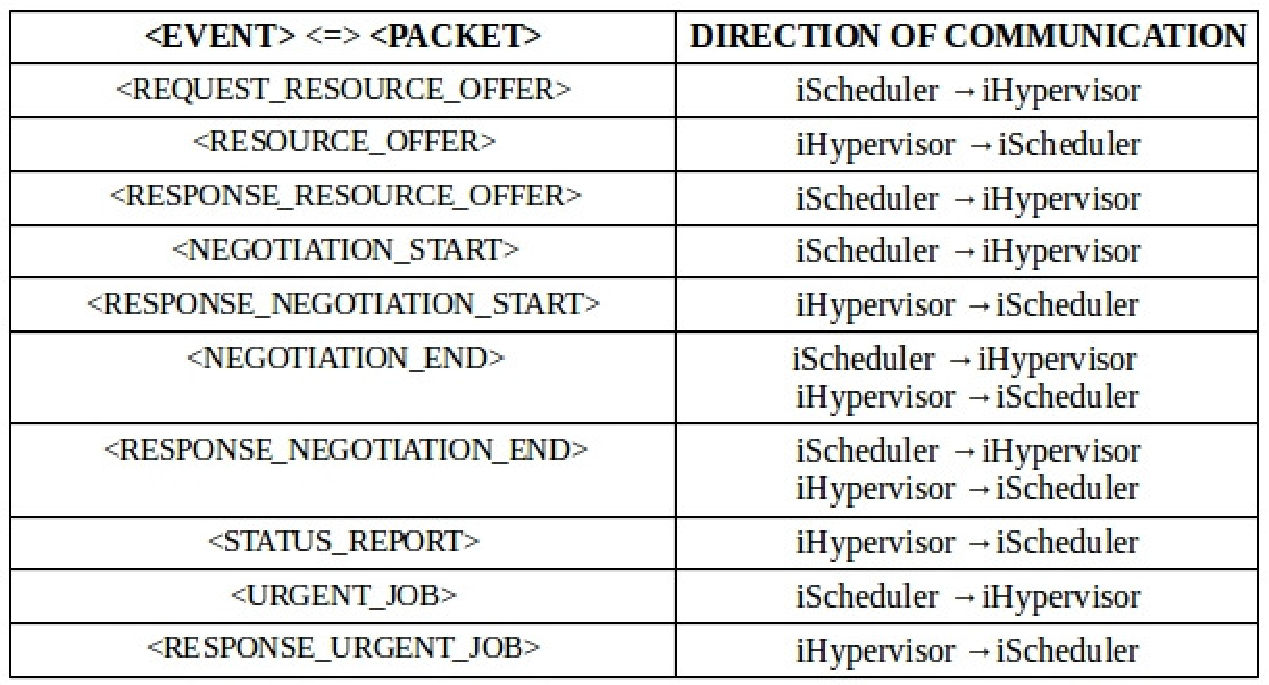
\includegraphics[width=1.0\textwidth, height=100mm]{./figures/table.pdf}
%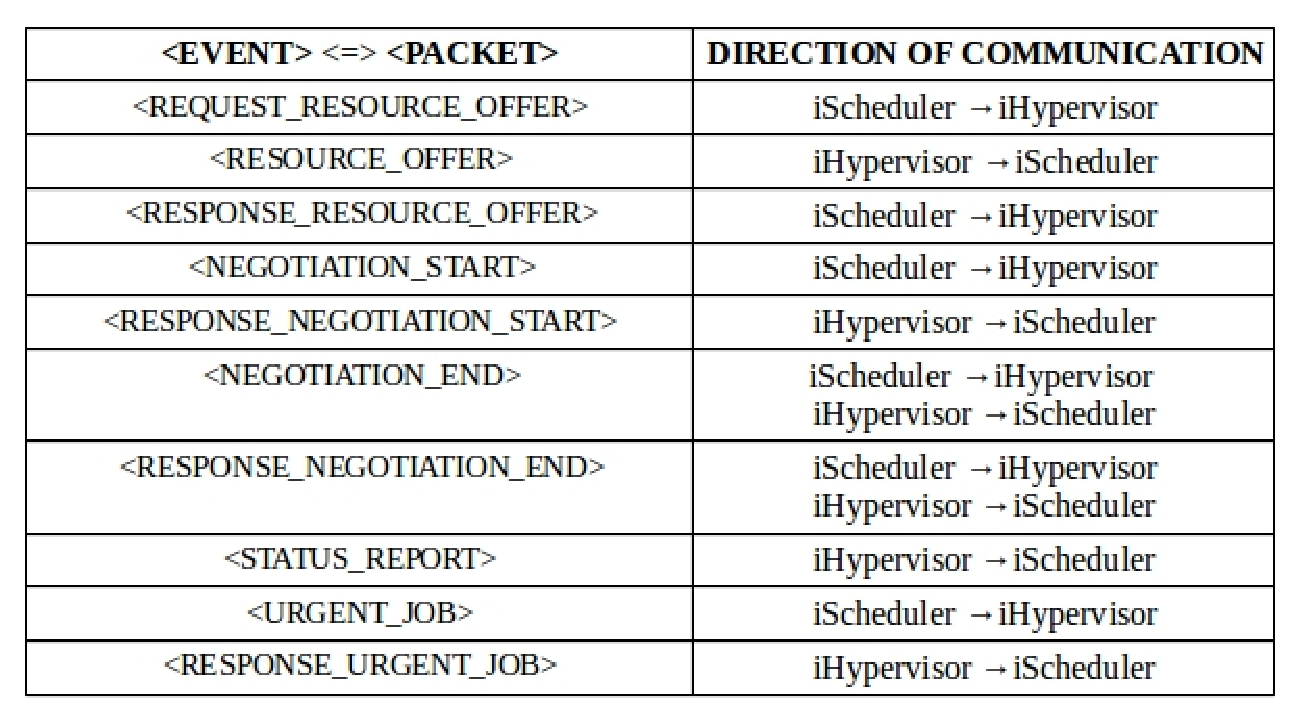
\includegraphics[width=1.0\textwidth, height=80mm]{./figures/table.eps}
\caption{Message Types}
\label{fig:8}
\end{figure}
\item \textbf{\textit{Negotiation:}} This is the most important phase in this whole approach to support invasive resource management. It is the phase during which both iRTSched and iBSched are negotiating with each other till they reach an agreement. If they do not then they continue till a certain limit is reached after which both of them just agree in their final attempt closing the current negotiation. After this a new transaction of negotiation will begin at some later point of time.
\item \textbf{\textit{Feedback:}} This concerns the periodic / event-driven feedback sent by the iRTSched to the iBSched containing useful information as mentioned earlier. iRTSched will also send a performance model of every completed job in the feedback that can be stored in some database as a part of the history of executions for this job. This will help the iBSched in the future if the same job is submitted when there will be additional performance specific information available about this job that can be used by the batch scheduling algorithm to make better decisions for this job. This protocol is a uni-directional communication.
\item \textbf{\textit{Urgent Jobs:}} This protocol concerns the support for urgent jobs. At any given point of time a cluster or supercomputing center may want to support very high priority jobs immediately without any further delay. By introducing support for invasive computing, it makes it all the more feasible to help run these urgent jobs immediately by either shrinking the resources of running jobs or suspending / killing them.
\end{itemize}
%%%%%%%%%%%%%%%%%
\section{Dynamic Resource Management}
\textbf{\textit{Separation of Concerns: }}In this thesis, We explore the idea of separating the concerns of batch and runtime scheduling into
two different software layers / components in contrast to the existing systems where both are merged together. A negotiation protocol will be implemented as a means of communication between the two. The motivation behind the negotiation protocol is the conflicting set of objectives between batch scheduler(user perspective: faster response time, fairness for jobs etc.) and run time scheduler(system perspective: maximize utilization, throughput, energy efficiency etc.). The role of the batch scheduler is to forward jobs to a runtime scheduler which is managing the resources in the partition(s) and supports runtime scheduling of jobs. Runtime scheduler will also make intelligent expand / shrink decisions by observing scalability behavior of the running applications which are adaptive and use it to predict future resource requirements. The proposed protocol will also allow us to integrate such adaptive resource management systems into existing batch systems and thereby allowing for an easy migration from legacy systems to invasive resource management systems. Negotiation also helps us to realize a dynamic and flexible scheduling strategy by balancing the conflicting objectives at the two layers.\\ \\
%%%%%%%%%%%%%%%
We will briefly look at the important components and their respective roles in this architecture in order to support adaptive applications on HPC systems by dynamically managing the resouce allocation of running jobs. 
\subsection{Invasive Batch Scheduler}
This component will be an extension to the batch scheduler in the existing batch systems. The scheduling decisions are communicated via the negotiation protocol to iRTSched. The scheduling decisions will be made on the basis of available resources in the partition and iRTSched communicates this to iBSched in the form of resource offers. Batch scheduler is making its decisions to optimize for certain local metrics such as reduced job waiting times, fairness, deadlines, priorities etc. The purpose of a batch scheduler is to select jobs from its queue according to some algorithm and dispatch this to the runtime scheduler. This is similar to a long term scheduler which by its definition: admits new processes to the system and controls the degree of multiprogramming( number of processes in memory). The batch scheduler for HPC workloads also does something similar but it is also merged with the runtime scheduler. In this work, we have separated the two because of which it now looks analagous to a long term scheduler(batch scheduler) that admits jobs into the HPC system and a short term scheduler(runtime scheduler) which will manage the running jobs. Batch scheduler runs less frequently and there may be quite a lot of time gap until the next job may be admitted into the system. This depends upon available resources, any events like job termination, completion where we can expect to receive a resource offer from the runtime scheduler.\\ \\
This batch scheduler is termed as invasive batch scheduler because it supports the negotiation interface to talk to an invasive run time scheduler. It will now consider a mix of job types which are: \textit{malleable, moldable, rigid, and evolving} and perform the following tasks as per the existing functionalities provided by SLURM:
\begin{itemize}
\item It is based on an event-driven batch scheduling where scheduling decisions would be made only when an offer is received from iRTSched. Scheduling is performed here at the granularity level of nodes.
\item Dispatch jobs according to a scheduling algorithm by considering the resource constraints of the job that can include the number[range] of nodes(exclusive / shared), memory size, duration, quality of service parameters etc.
\item With every negotiation attempt, the batch scheduler will try to relax the constraints of those jobs which could not be mapped to the available resource offer. As the negotiation attempts increase the degree to which the constraints are relaxed also increases. By doing this the batch scheduler is trying to bargain as best as it can in order to get an offer to serve as many jobs as possible.
\item It will process the feedbacks received from iRTSched and update the job details in the queue such that it is visible to the administrator.
\item It can also process jobs which have an urgent priority. These jobs will receive special service and are going to be dispatched immediately to iRTSched. It will also consider jobs that may have some quality of service requirements such as deadlines and start time.
\item Based on the the offers received from the iRTSched, the batch scheduler may try to bias its scheduling decisions towards certain jobs(io/cpu bound).
\item If a job that is in the queue has already been submitted in the past and there is some history stored in the system about it, Then the batch scheduler will use the history information from the database to update the job details. This can lead to better scheduling decisions for this job.
\end{itemize}
\subsection{Invasive Run Time Scheduler}
This is an independent component which can talk to the existing batch systems via a negotiation protocol to receive forwarded batch jobs for execution. The runtime scheduler manages the running jobs via space sharing, time sharing or both. The runtime scheduler here is invasive because of the ability to support elastic execution for jobs that are adaptive. It can now redistribute resouces to running jobs by either expanding or shrinking them based on their performance and scalability. Following points describe the role of iRTSched:
\begin{itemize}
\item It manages all the resources in the partition and is responsbile for runtime scheduling at the granularity of cores / sockets, resource management and process management(infrastructure to launch, adapt and monitor parallel jobs).
\item It will use an intelligent expand / shrink algorithm to dynamically adjust the resources of running jobs which are adaptive in nature. 
\item Runtime scheduler will bias its decisions towards maximizing throughput, energy efficiency, optimize for topology, resource utilization etc.
\item Similar to iBSched, iRTSched will increase the degree of transformation of the runtime state of the system to better serve the batch scheduler. As the negotiation attempts increase, the scheduler will try its best to fit every batch job forwarded by performing an aggressive transformation of the running jobs. Aggressive here means that the scheduler will try to either expand / shrink jobs to their maximum / minimum.
\item In addition to expand / shrink strategy, The runtime scheduler can support scheduling algorithms like backfilling, gang scheduling, preemption etc.
\item iRTSched will build a performance model of the running application or will refine an existing model if it was forwarded by the batch scheduler in the job details. It will also make its scheduling decisions using this performance model to estimate the scalability, performance and efficiency of the application at different job sizes.
\item It will send the generated models and other relevant information about a completed job like runtime, energy consumption, IO consumption in a feedback report to the iBSched.
\item Runtime scheduler can send resource offers to batch scheduler for the following events: job termination, job completion, request for a resource offer, periodic runtime transformations of running jobs resulting in free resources.
\end{itemize}
\subsection{iMPI Process Manager}
The iMPI process manager in this architecture refers to multiple components as they all are necessary to successfully provide an elastic execution framework for adaptive applications. These components are \textbf{\textit{srun}}, \textbf{\textit{slurmd}} and \textbf{\textit{slurmstepd}}. The previous chapter already described as to how the extended MPI library called as iMPI allows the programmer to create invasive MPI applications and how the extensions on the resource manager side in coordination with iMPI provide a complete infrastructure necessary for the elastic execution of adaptive applications.
\section{Negotiation Protocol}
This protocol forms the core of the interaction between the iBSched and iRTSched. It allows for iRTSched to make one or a set of resource offers to iBSched which then needs to select jobs from its job queue to be mapped to these resource offers and send back the mapping to the iRTSched. The iRTSched will then decide whether to accept/reject this mapping based on whether it satisfies its local metrics. If it accepts it will launch them based on some run time scheduling and if it rejects then it informs this to iBSched in addition to sending it a new resource offer
that will also contain possible future start times for pending jobs. The iBSched can also reject the resource offer in which case it will forward the previous job mapping(if any) again with relaxed resource constraints for jobs that could not be mapped. On accepting an offer, the iBSched will again send back a mapping to iRTSched. This exchange of messages continue until both reach an agreement. If the number of such exchanges reach a threshold then iBSched will just accept whatever offer it receives and iRTSched will also accept the final mapping it received and try its best to satisfy all the jobs forwarded. This will close the transaction.
\subsection{Protocol Sequence Diagrams}
%\vspace{-0.15in}
\begin{figure}[!t]
%\begin{figure}[H]
\centering
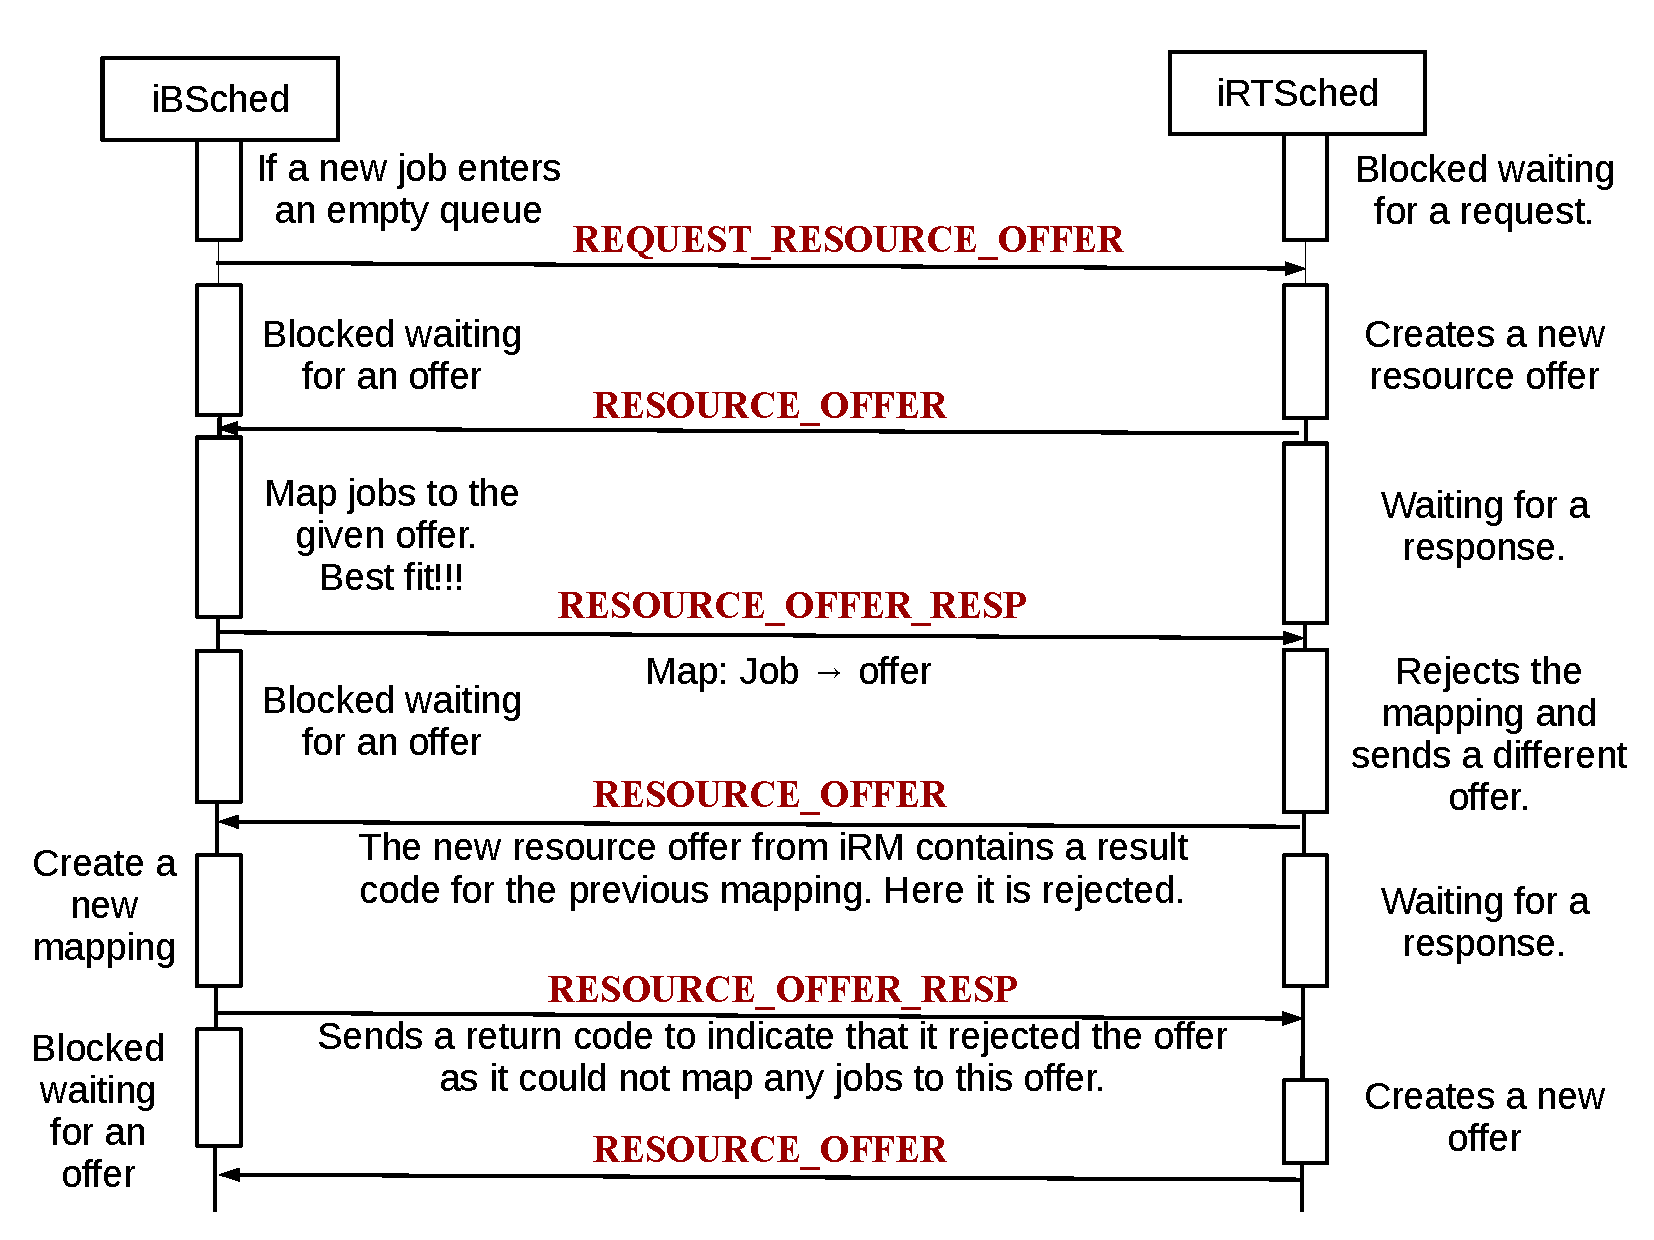
\includegraphics[width=1.0\textwidth, height=100mm]{./figures/scenario1.pdf}
%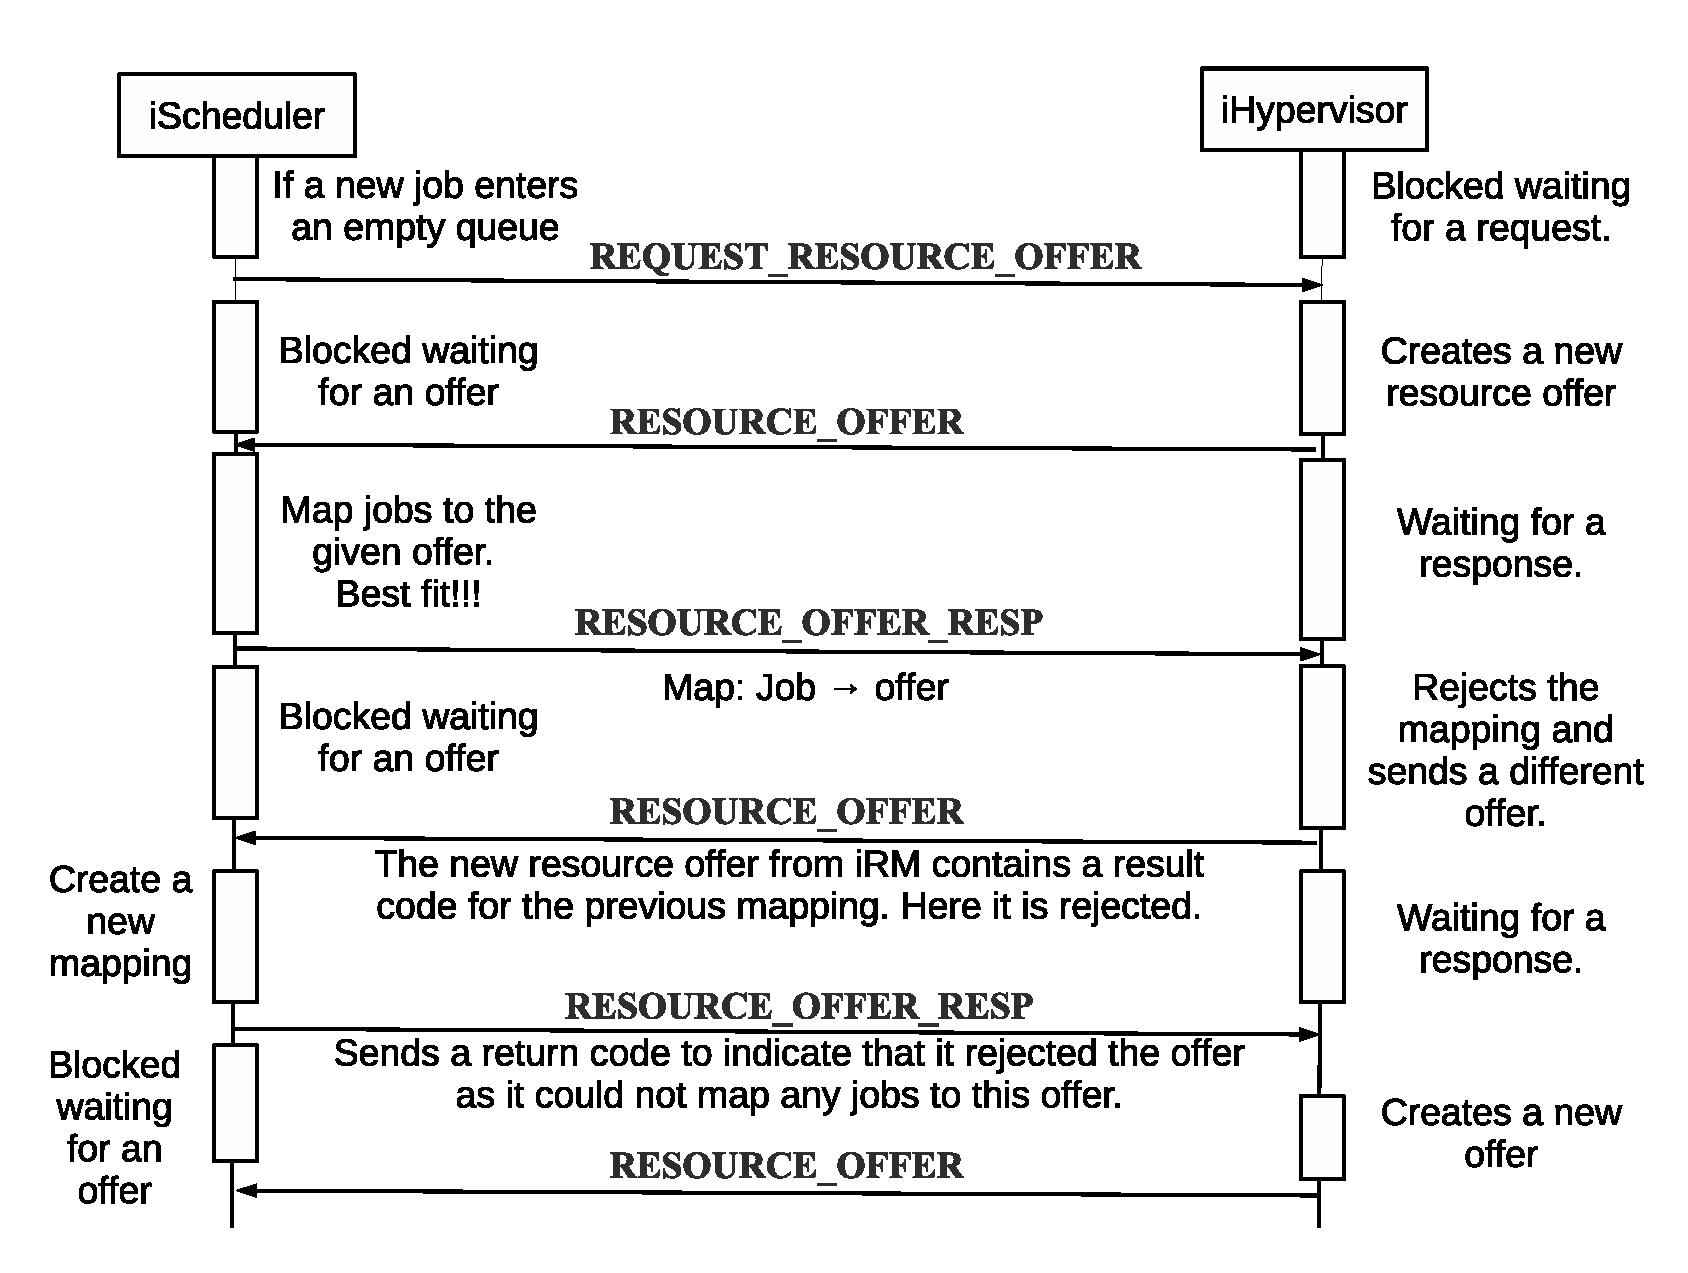
\includegraphics[width=1.0\textwidth, height=100mm]{./figures/figures.eps}
\caption{Scenario 1}
\label{fig:Seq1}
\end{figure}
\begin{itemize}
\item Figure \ref{fig:Seq1} illustrates a scenario where both iBSched and iHpervisor are negotiating with each other. The scenario is continued in the figure \ref{fig:Seq2}. Figure \ref{fig:Seq3} illustrates another scenario where negotiations may stop when job queue becomes empty and iHypevisor then will wait for a request from iBSched for a resource offer that will happen when new jobs arrive.
\item iBSched makes scheduling decisions at a coarser level of granularity which is nodes whereas iRTSched does at the granularity of cores and sockets. Both will negotiate with each other till they reach an agreement.
\item It is an event based scheduling which means iBSched makes a scheduling decision only when it is triggered by receiving a resource offer from iRTSched. It is only when the invasive job queue becomes empty that iBSched will have to explicitly send a request message to iRTSched for a resource offer otherwise at all other times scheduling is event based.
\end{itemize}
%\label{fig:Seq1}
%\end{figure}
\begin{figure}[!t]
\vspace{-0.25in}
\centering
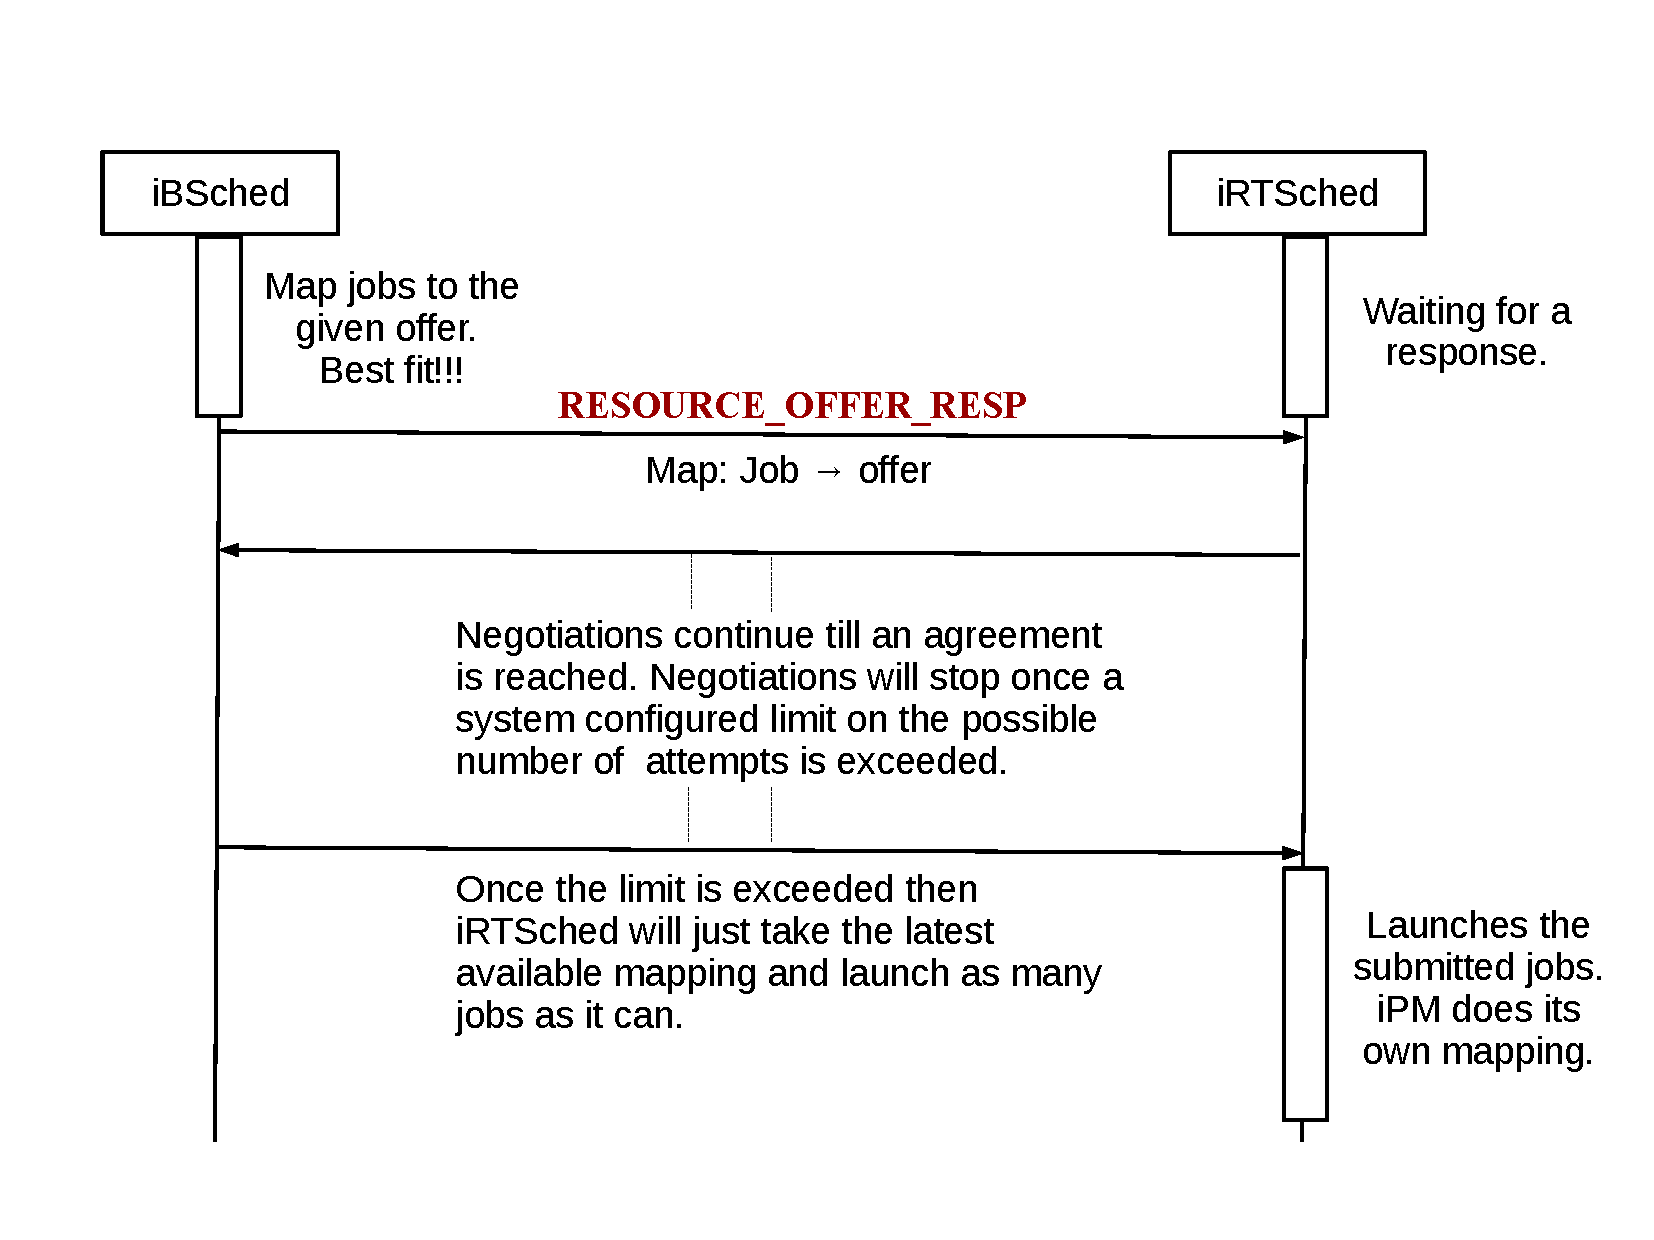
\includegraphics[width=0.9\textwidth, height=90mm]{./figures/scenario1contd.pdf}
%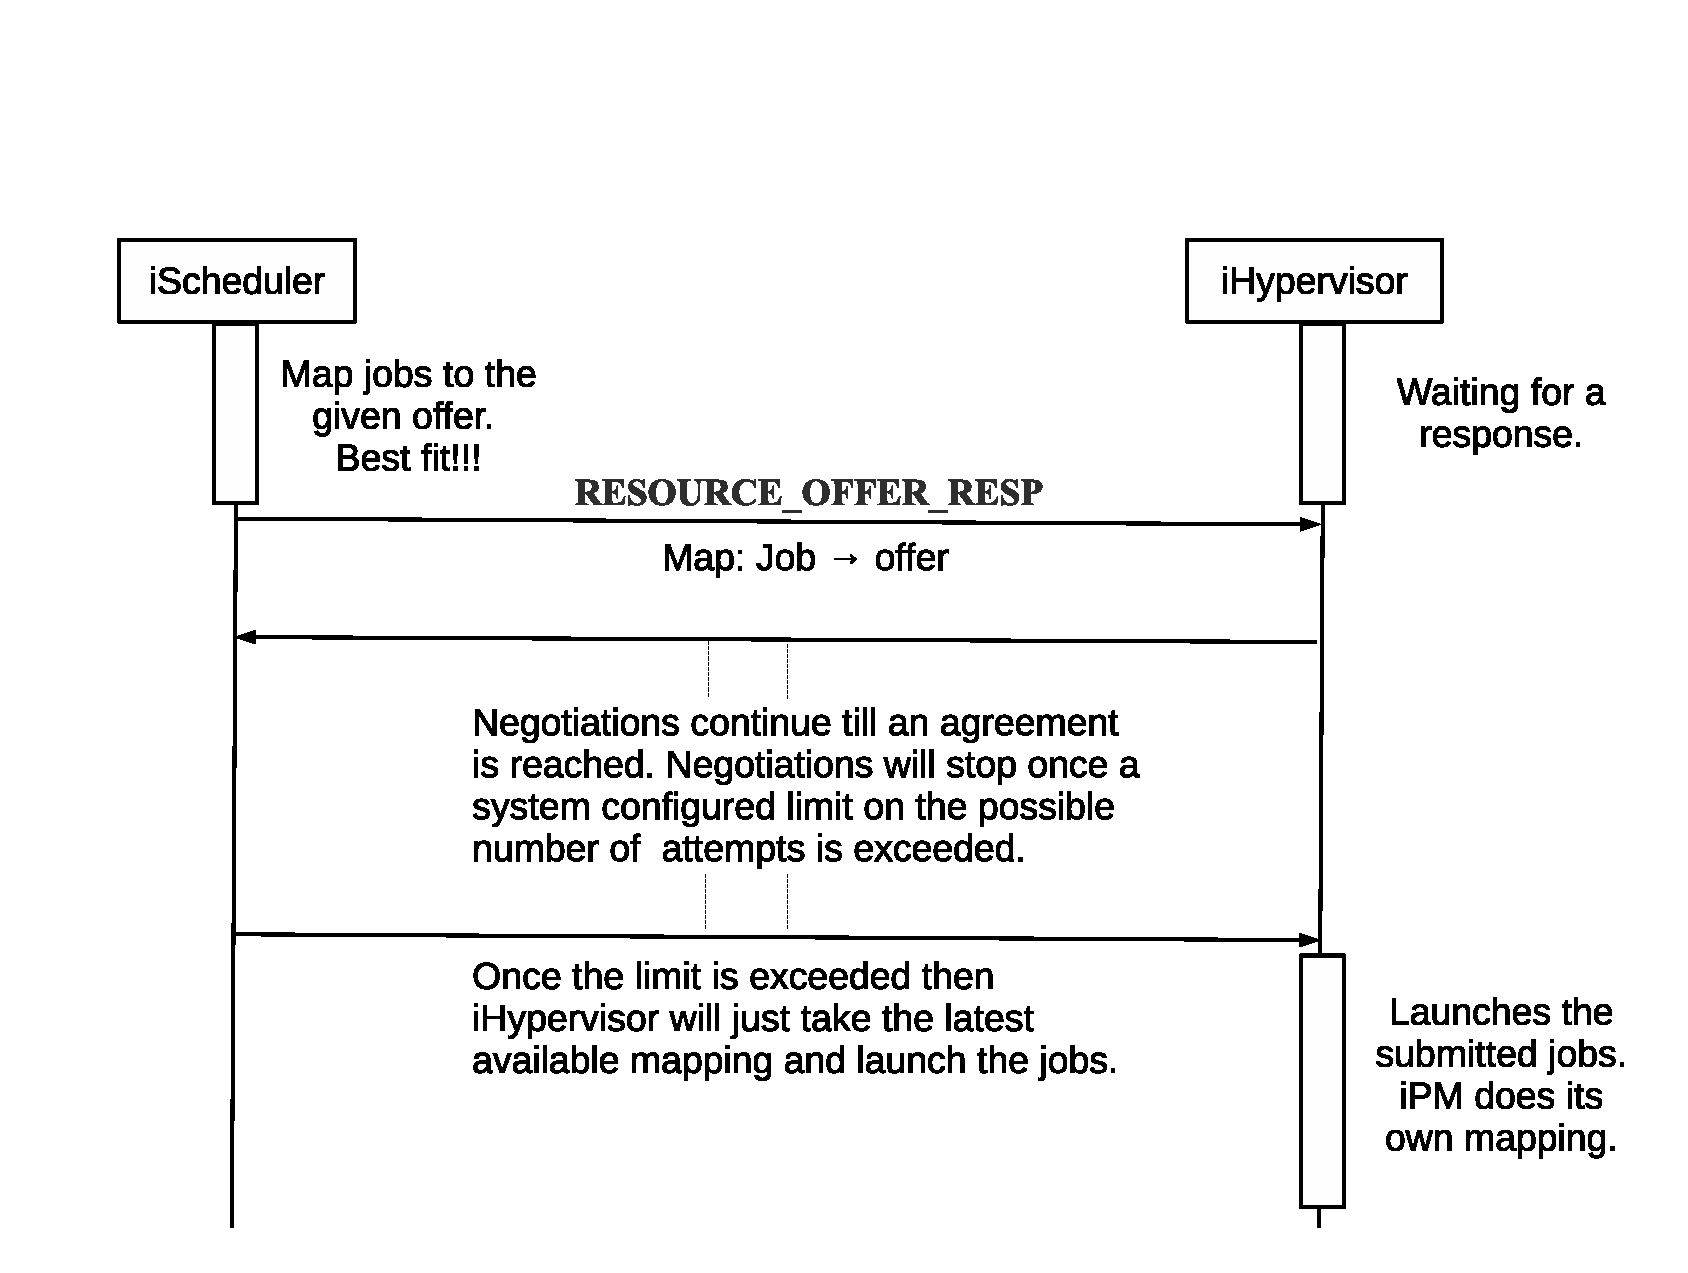
\includegraphics[width=0.9\textwidth, height=100mm]{./figures/figures1.eps}
\caption{Scenario 1 contd.}
\label{fig:Seq2}
%\vspace{-0.10in}
\end{figure}
\begin{figure}[!b]
%\vspace{-0.15in}
\centering
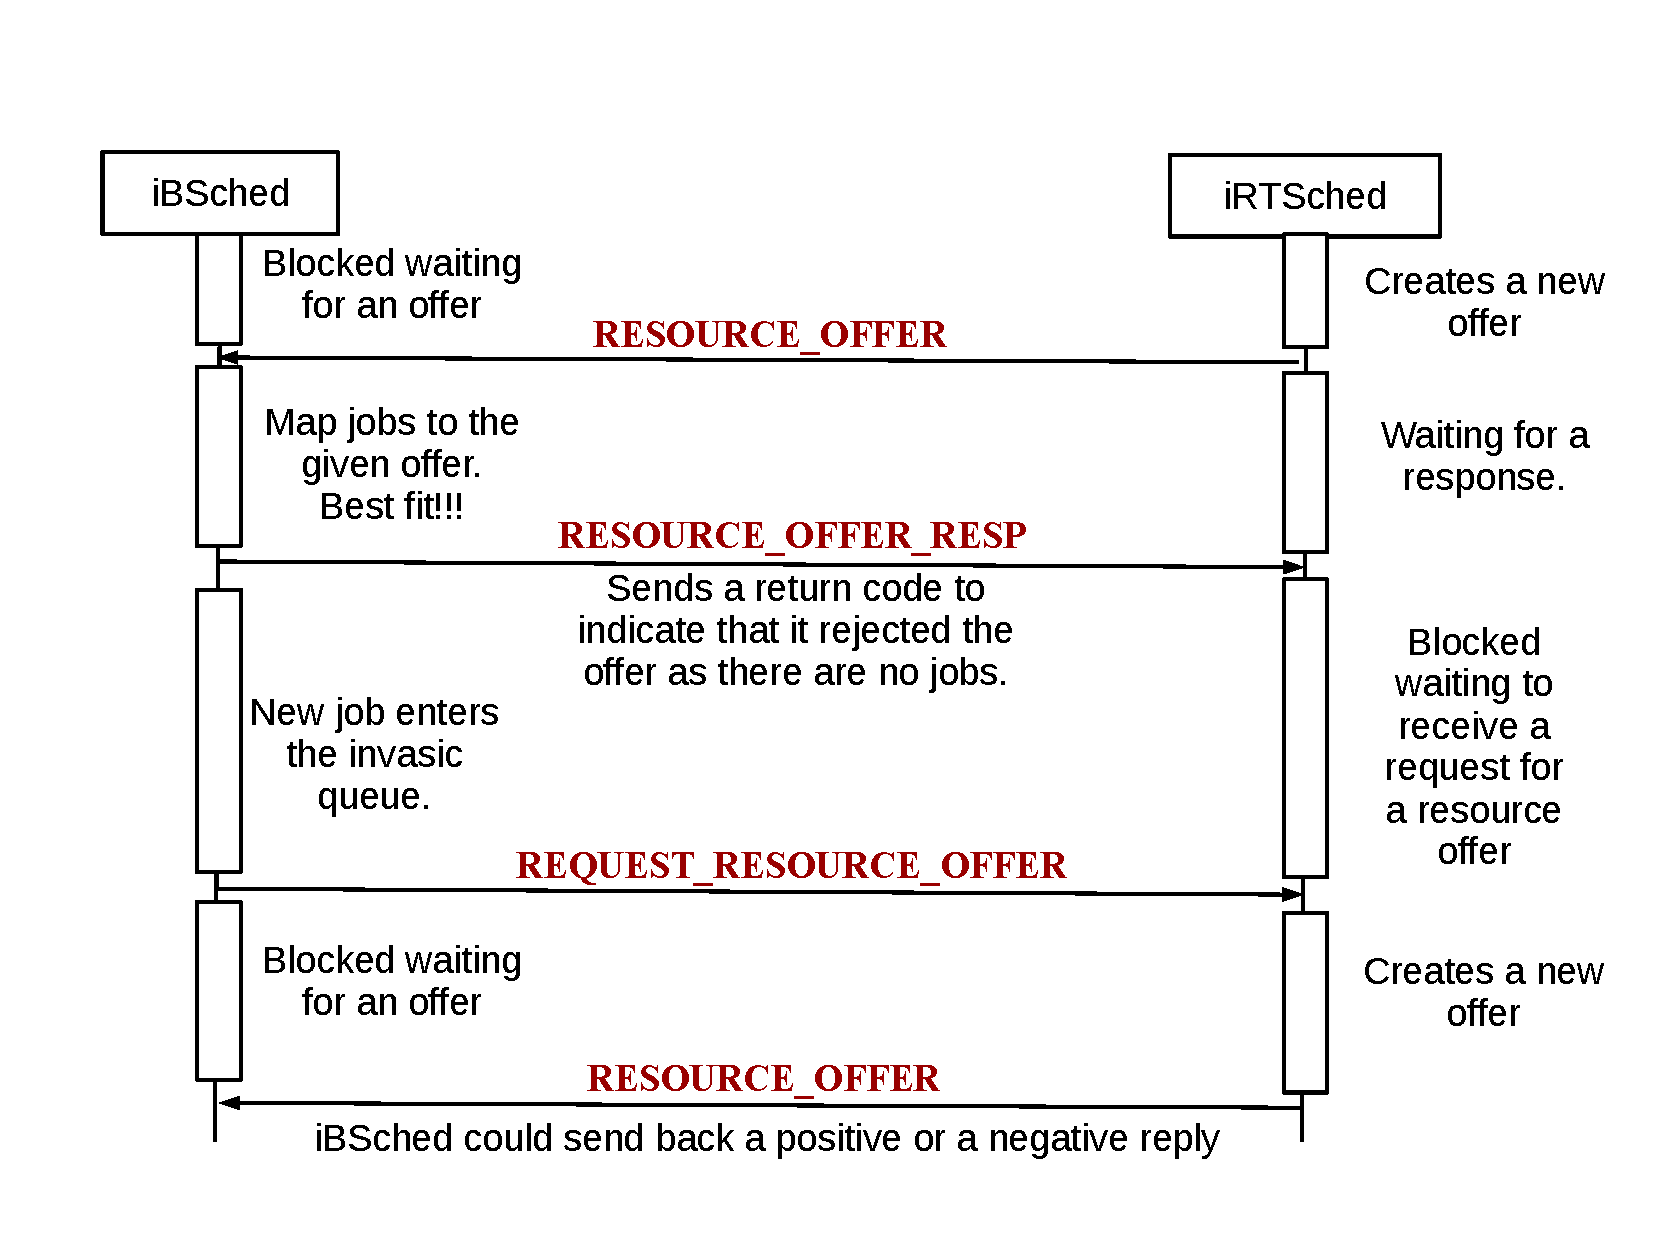
\includegraphics[width=0.9\textwidth, height=90mm]{./figures/scenario2.pdf}
%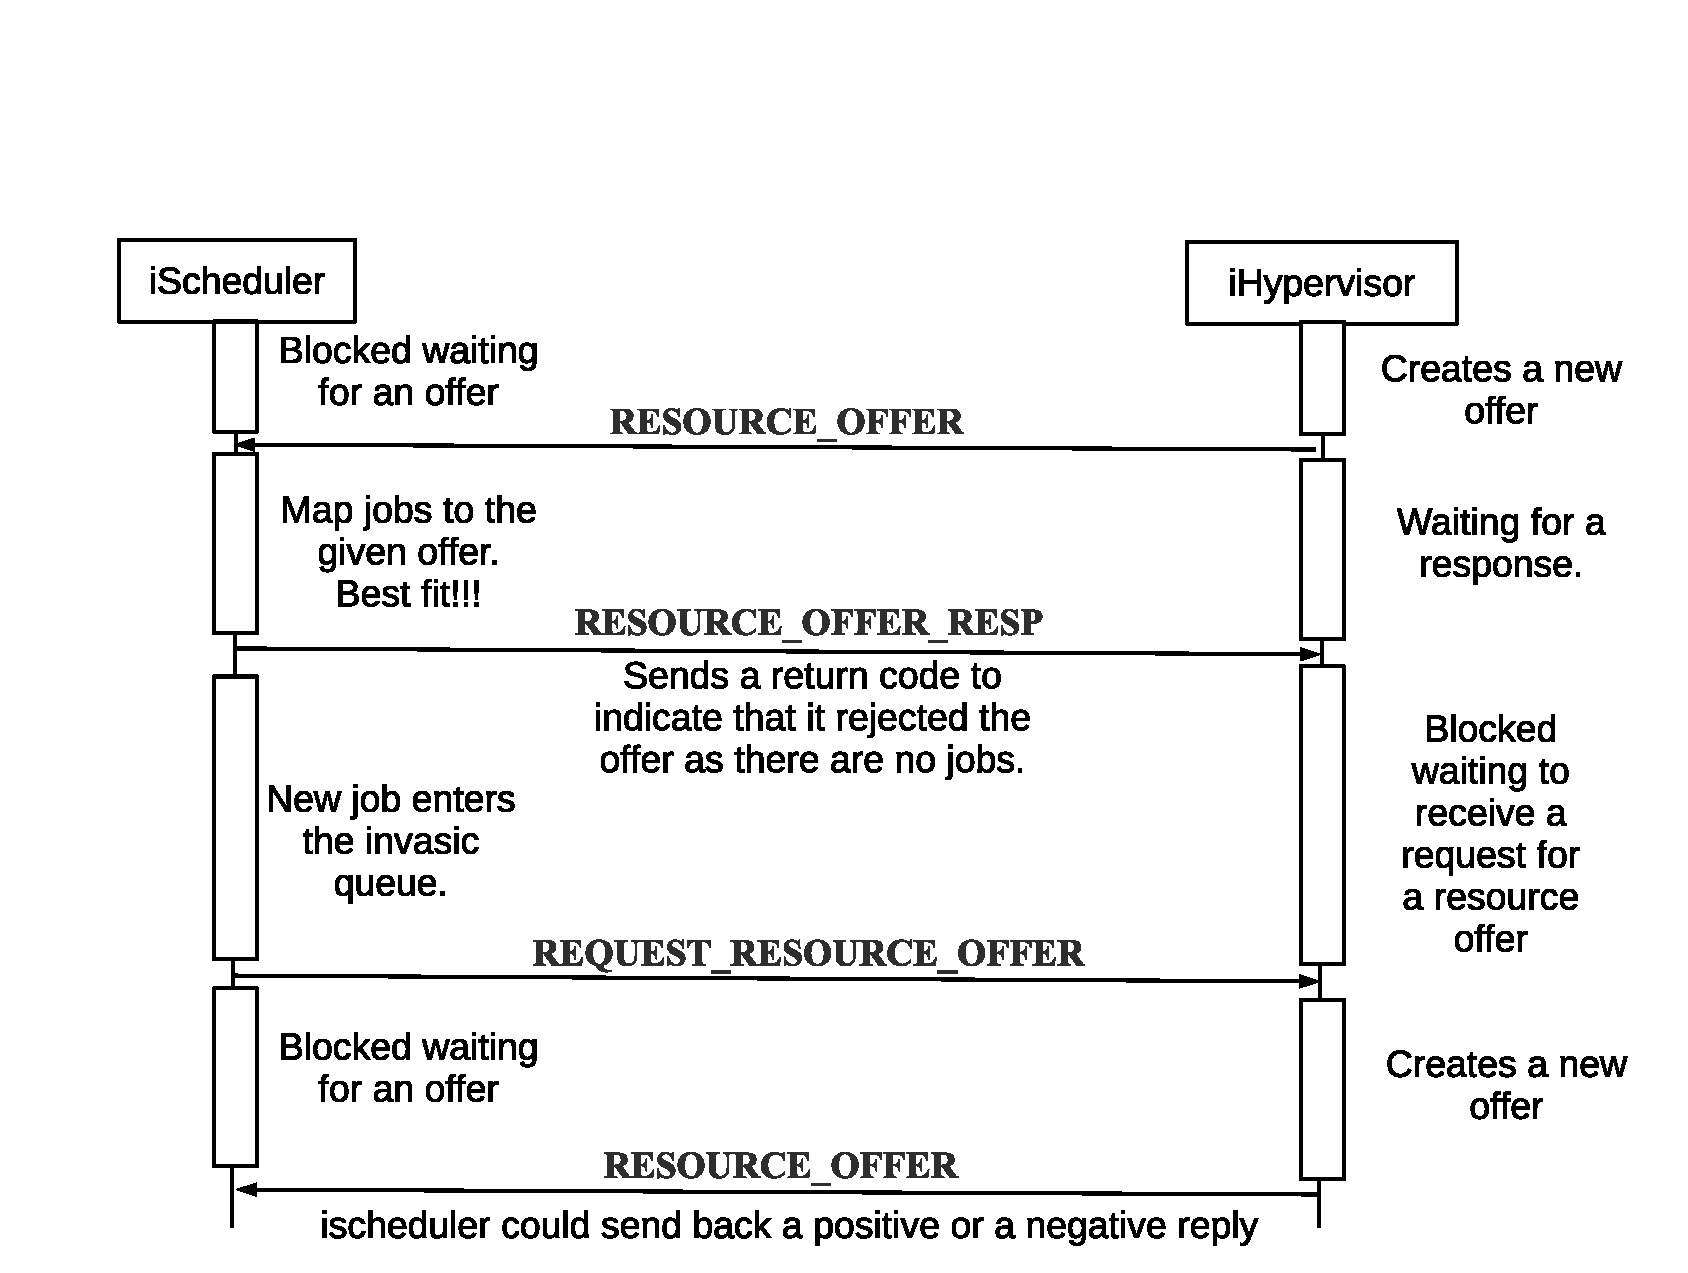
\includegraphics[width=0.9\textwidth, height=100mm]{./figures/figures2.eps}
\caption{Scenario 2}
\label{fig:Seq3}
\end{figure}
\section{Invasive Jobs}
Invasive jobs refer to those jobs whose resource set can be changed at runtime. As mentioned before in the job classification, \textbf{\textit{malleable}} and \textbf{\textit{evolving jobs}} fall under this category and we will refer to these as invasive jobs in the report. These kind of jobs will usually come with a set of constraints when submitted to a HPC system. An example of how such constraints may look like is given below. Some of these constraints will already be supported by current batch systems for job submission.\\ \\
\textbf{\textit{Node Count:}} <min nodes><max nodes>\\
\textbf{\textit{Runtime Estimate:}} <duration for min nodes>\\
\textbf{\textit{Memory Per Node:}} <min MB>\\
\textbf{\textit{Hint:}} <io bound | cpu bound | communication bound | na>\\
\textbf{\textit{Urgent:}} <yes | no> \\
\textbf{\textit{Deadline:}} <timestamp | na>\\
\textbf{\textit{Start Time:}} <timestamp | na>\\
\textbf{\textit{Budget:}} <core hours>\\
\textbf{\textit{Performance Model:}} <if available>\\ \\
na $\rightarrow$ not available
